\section{Theorie}

%Was ist Beugung(Einzelspalt, Gitter, Aperturfunktion, Sinusgitter, Fouriertrafo)
%Laser (nur Eigenschaften)

\subsection{Beugung}

\subsubsection{Allgemeine Definition}

Als Beugung bezeichnet man das Ph\"anomen, dass Licht, welches durch begrenzende \"Offnungen oder an begrenzenden Kanten vorbeil\"auft, von seiner urspr\"unglichen Richtung abgelenkt wird. Hinter dem Hindernis \"uberlagern sich die Teilwellen gem\"a\ss dem Huygenschen Prinzip, welches besagt, dass jeder Punkt einer Wellenfront eine neue Welle induziert. Diese \"uberlagern sich dann und die daraus resultierenden Interferenzerscheinungen werden als Beugung bezeichnet.

\subsubsection{Das Kirchhoff'sche Beugungsintegral}

\begin{figure}[H]
	\centering 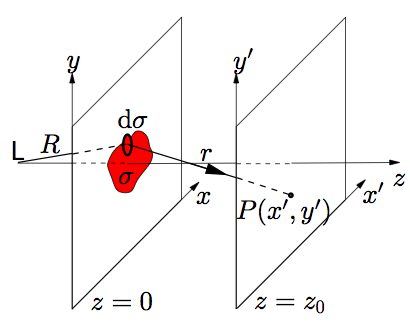
\includegraphics[width=0.5\textwidth]{Bilder/Beugungsintegral.jpg}
	\caption{Zum Kirchhoffschen Beugungsintegral}
\end{figure}

Licht mit der Amplitude $E_\sigma$, welches auf die Blenden\"offnung $\sigma$ f\"allt, hat im Punkt $P$ auf dem Schirm hinter der \"Offnung die Amplitude: $$dE_P = C\frac{E_\sigma \cdot d\sigma}{r}e^{-ikr}$$
($C$ ist hier ein Proportionalit\"atsfaktor)\\
Betrachtet man die Beitr\"age aller $d\sigma$, so erh\"alt man das Fresnel-Kirchhoffsche Beugungsintegral:
$$E_P=\iint C\cdot E_\sigma \cdot \frac{e^{-ikr}}{r}dxdy$$

Dieses Integral kann man nun mit der Fraunhofer-N\"aherung als Fourierintegral umwandeln. Die Fraunhofer-N\"aherung ist eine Fernfeldn\"aherung; die Spaltgr\"o\ss e wird als klein angenommen und die Lichtquelle als sehr weit entfernt. Mit diesen Vereinfachungen wird das Integral zu:

$$ E(x',y') = A(x',y',z_0)\cdot \iint E_{ein}(x,y)\cdot g(x,y)\cdot \exp(-i2\pi(x'x+y'y)/(\lambda z_0)) dxdy $$

und es gilt der Zusammenhang:

$$ E(x',y',z_0) = F(u,v) \cdot A(x',y',z_0)$$

wobei \begin{itemize}
\item $F(u,v)$ das Fourierintegral der Funktion $f(x,y) = g(x,y)\cdot E_{ein}(x,y)$
\item $g(x,y)$ die Aperturfunktion der \"Offnung
\item $A(x',y',z_0)=\frac{e^{-ikz_0}}{i\lambda z_0}\cdot e^{i\pi (x'^2 + y'2) / \lambda z_0}$ und $|A|^2 =1$
\end{itemize}

Somit folgt f\"ur die Intensit\"at:

$$I \sim |E|^2 = \iint g(x,y)\cdot e^{ikr} dxdy$$


\subsubsection{Anwendungen}

\begin{enumerate}
 
\item Beugung am Einzelspalt


\begin{minipage}{0.6\textwidth}
Die Aperturfunktion am Einzelspalt (unter Vernachl\"assigung der Begrenzung in y-Richtung) lautet
$$ g(x) = \begin{cases} 
	1 & \text{, falls} -\frac{b}{2}<x<\frac{b}{2}\\
	0 & \text{, sonst}
     \end{cases}$$
Man erh\"alt durch Ausrechnen des Beugungsintegrals folgende Abh\"angigkeit f\"ur die Intensit\"at:
$$ I \sim \left(\frac{\sin(\beta)}{\beta}\right)^2 $$
\end{minipage}
\begin{minipage}{0.4\textwidth}
	\begin{center}
		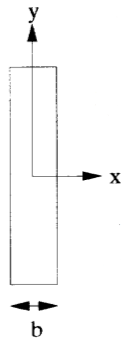
\includegraphics[width=0.35\textwidth]{Bilder/Einzelspalt.jpg}
	\end{center}
\end{minipage}

Hier ist $\beta = \frac{k}{2b}\sin(\theta)$ und $\theta$ der Einfallswinkel auf dem Schirm vom Ursprung des Spaltes aus.

\item Beugung am Gitter

\begin{minipage}{0.6\textwidth}
Ein Gitter besteht aus N Einzelspalten nebeneinander angeordnet. Alle Spalten haben idealerweise die Breite $b$ und die Distanz $K$ voneinander in $x$-Richtung.
\end{minipage}
\begin{minipage}{0.4\textwidth}
	\begin{center}
		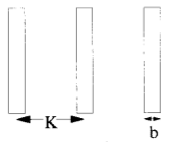
\includegraphics[width=0.7\textwidth]{Bilder/Gitter.jpg}
	\end{center}
\end{minipage}



\end{enumerate}















